\documentclass[aspectratio=169]{beamer}
\usepackage{UFtheme}
%% ===========================================
%% ===========================================
\title{\LARGE \textbf{Lec 7: Uncertainty Estimation, Bayesian Inversion, and Future Directions} \vspace{0.2cm}}
\author{GEOM-S2091 Inversion of Geophysical data }

\date{\small \today}
%% ===========================================
%% ===========================================
\begin{document}
\begin{frame}[plain]
    \titlepage
\end{frame} 
%% ===========================================    
%% ===========================================

% Uncomment these lines for an automatically generated outline.
%\begin{frame}{Outline}
%  \tableofcontents
%\end{frame}


%% ===========================================
%% ===========================================
%	PRESENTATION SLIDES
%% ===========================================
%% ===========================================

%% ===========================================
%% ===========================================
\section{Motivation} 

\subsection{Subsection Example} % A subsection can be created just before a set of slides with a common theme to further break down your presentation into chunks

%% ===========================================
%% ===========================================





\begin{frame}{\textbf{Motivation}}
 \begin{figure}
\centering
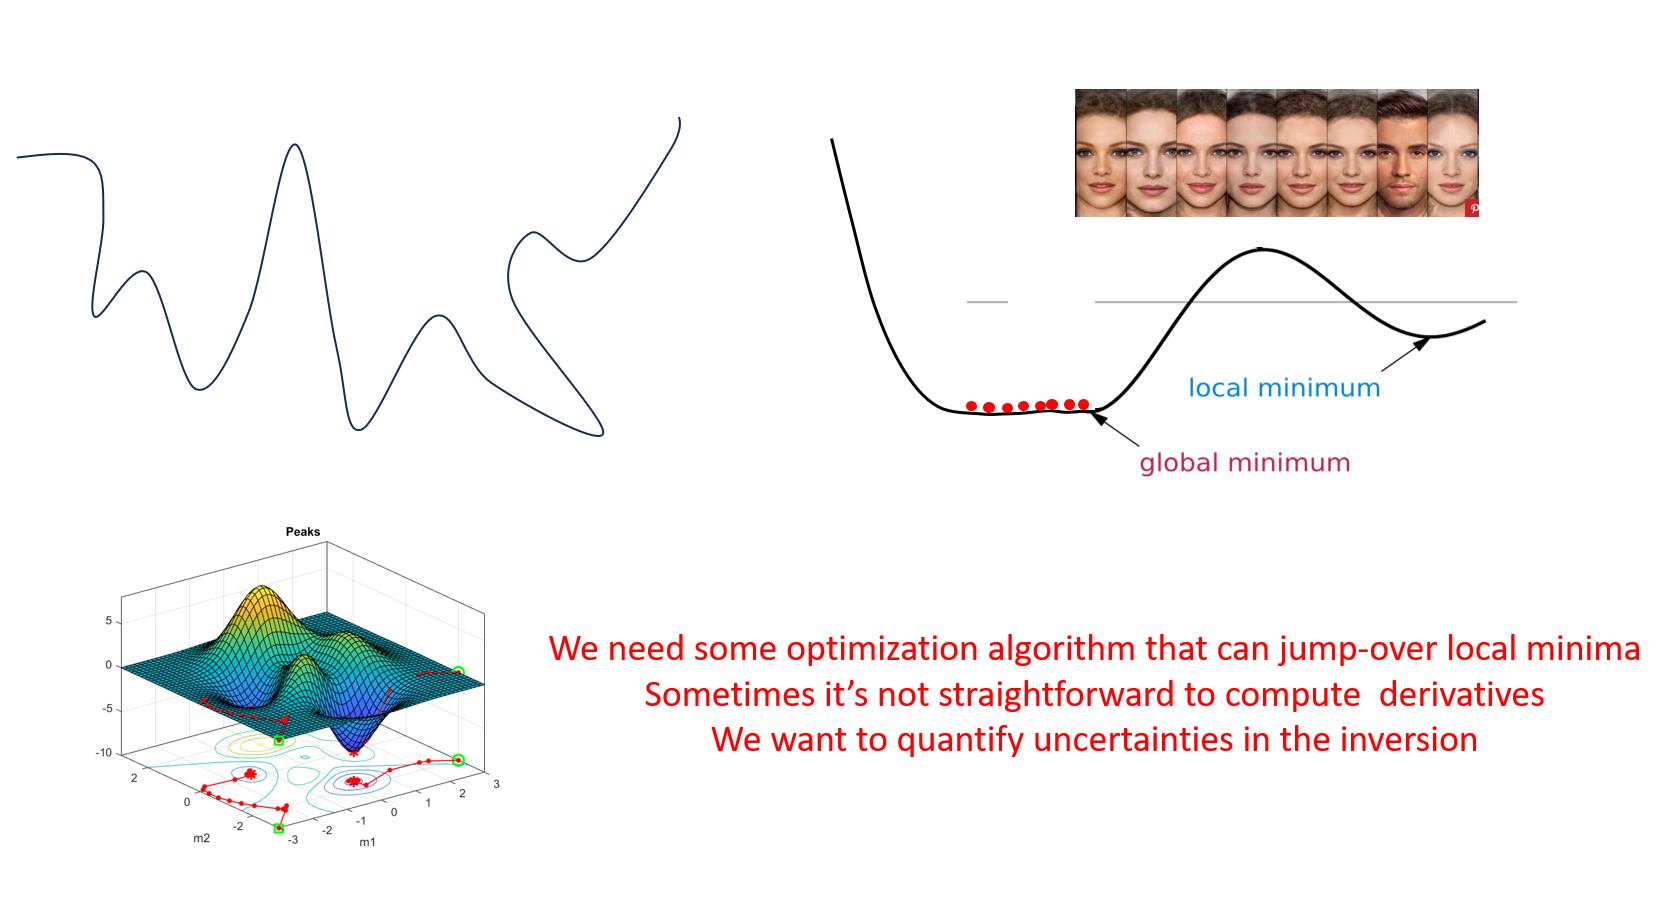
\includegraphics[scale=0.35]{Figures/motivation.PNG}
\end{figure}   
\end{frame}



\begin{frame}{\textbf{Uncertainty Estimation is important}}
 \begin{figure}
\centering
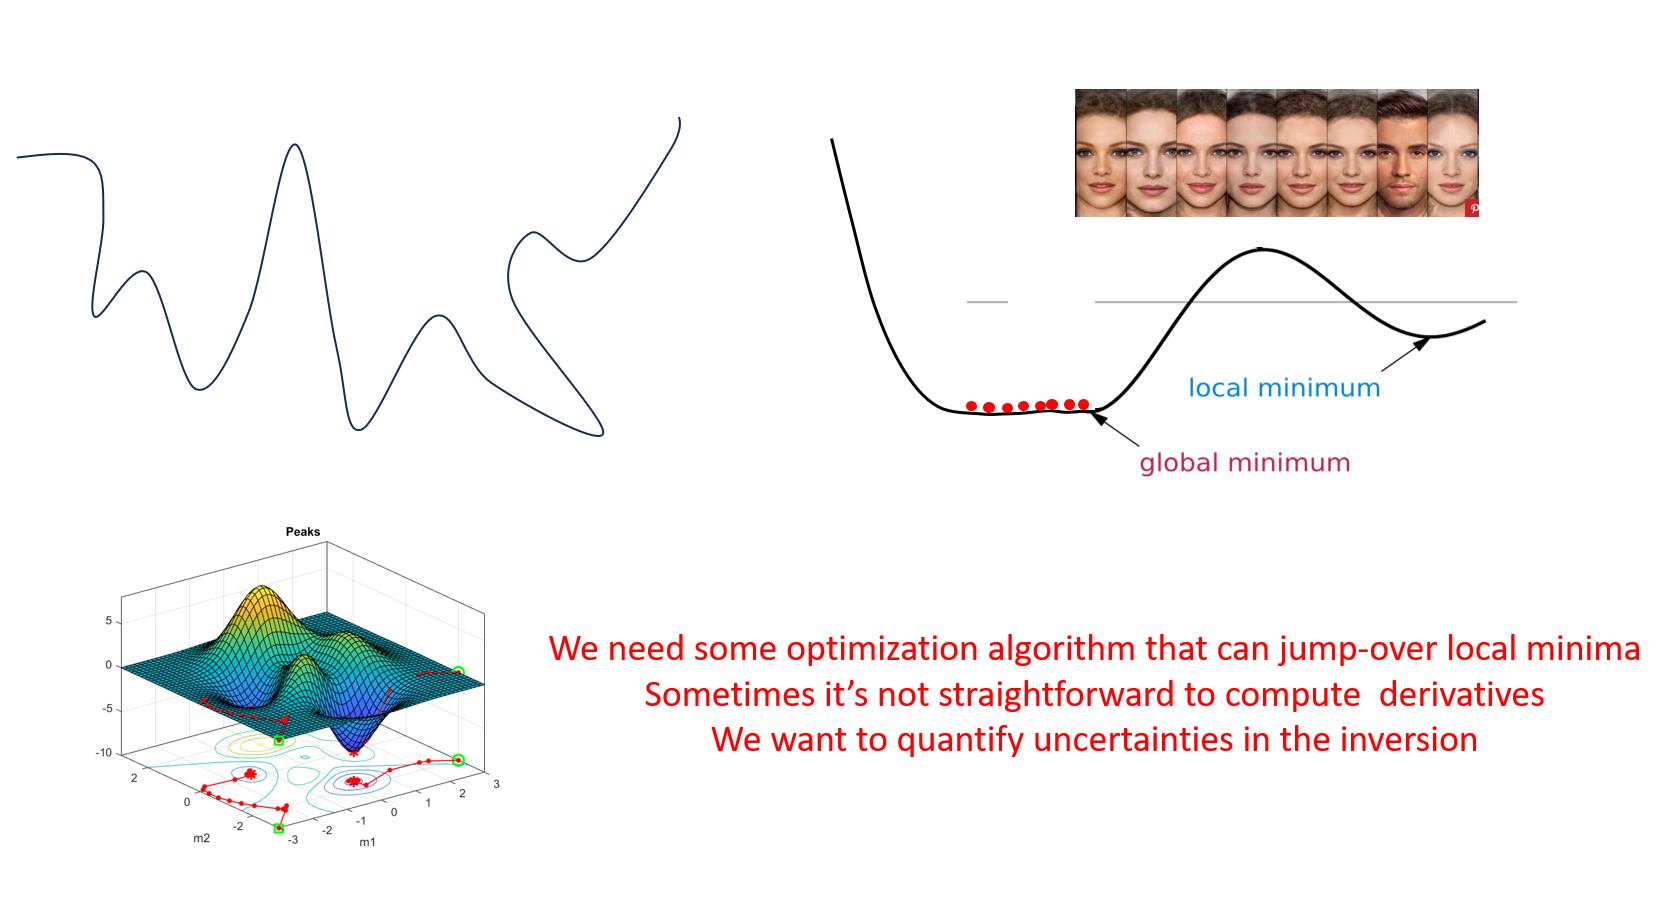
\includegraphics[scale=0.35]{Figures/motivation.PNG}
\end{figure}   
\end{frame}









%% ===========================================
\section{Probability review} 
\subsection{}
\begin{frame}
\frametitle{\textbf{Random Variables}}
\begin{itemize}
    \item [$\bullet$] Random variables describe the outcomes of statistical experiments numerically.
    \item [$\bullet$] Types of random variables:
    \begin{enumerate}
        \item Discrete Random Variables
        \item Continuous Random Variables
    \end{enumerate}
\end{itemize}
\end{frame}


\begin{frame}
\frametitle{\textbf{Discrete Random Variables in a Classroom}}
\begin{itemize}
    \item [$\bullet$] \textbf{Quiz Scores:}
    \begin{itemize}
        \item [$-$]  Possible scores on a 10-question quiz: 0, 1, 2, ..., 10.
        \item [$-$]  Each score represents a discrete outcome.
    \end{itemize}
    \item [$\bullet$] \textbf{Attendance Count:}
    \begin{itemize}
        \item [$-$] Count of students present any day: 0 to total number enrolled.
        \item [$-$] Each count is a possible outcome of the random variable.
    \end{itemize}
\end{itemize}
\end{frame}


\begin{frame}
\frametitle{\textbf{Continuous Random Variables in a Classroom}}
\begin{itemize}
    \item [$\bullet$] \textbf{Time Spent on Homework:}
    \begin{itemize}
        \item [$-$] Time can vary continuously (e.g., 30.5 minutes, 45.75 minutes).
        \item [$-$]  Measured as a continuous random variable.
    \end{itemize}
    \item [$\bullet$] \textbf{Height of Students:}
    \begin{itemize}
        \item [$-$]  Height measured to any level of precision (e.g., 162.4 cm).
        \item [$-$]  Represents a continuous measurement.
    \end{itemize}
\end{itemize}
\end{frame}


\begin{frame}
\frametitle{\textbf{Probability Distributions}}
A probability distribution describes how the values of a random variable are distributed. It is a mathematical description of the probabilities of occurrence of different possible outcomes in an experiment.
 \begin{itemize}
        \item [$\bullet$]\textbf{Non-negativity:} \( p(x) \geq 0 \) for all \( x \).
        \item [$\bullet$] \textbf{Total area equals 1:} The total area under the curve of the PDF across the entire range is 1. Mathematically, \( \int_{-\infty}^{\infty} p(x) \, dx = 1 \).
    \end{itemize}

    \textbf{Example: Normal Distribution PDF}
    \begin{itemize}
        \item [$-$] The Normal (Gaussian) Distribution is a common continuous probability distribution, often represented by:
        \[
        p(x|\mu,\sigma) = \frac{1}{\sigma\sqrt{2\pi}} e^{-\frac{(x-\mu)^2}{2\sigma^2}}
        \]
        where \( \mu \) is the mean  and \( \sigma \) is the standard deviation of the distribution.
    \end{itemize}

\end{frame}


\begin{frame}{\textbf{Various PDFs}}
 \begin{figure}
\centering
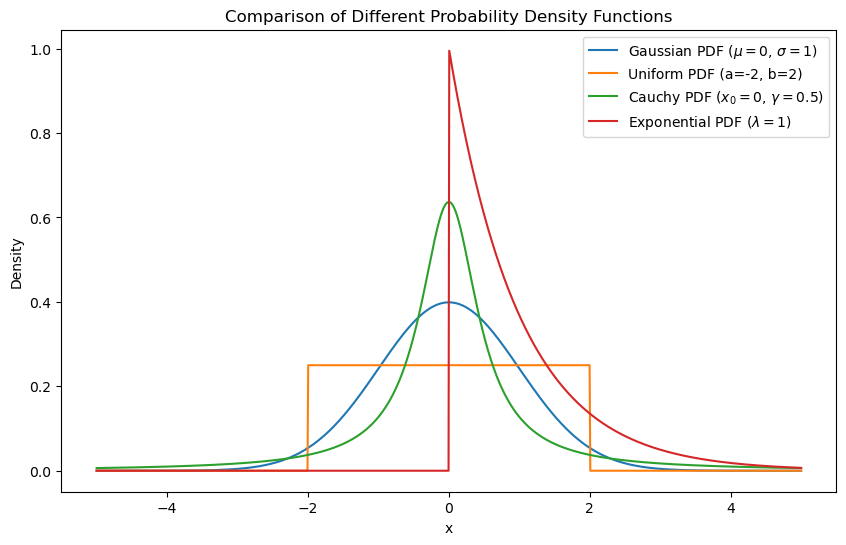
\includegraphics[scale=0.5]{Figures/plot_PDFs.png}
\end{figure} 
\end{frame}


\begin{frame}{\textbf{Using PDF }}
The probability that a random variable M is between $a$ and $b$ is the area under the curve between $a$ and $b$. 
\[
P(a \leq X \leq b) = \int_{a}^{b} p(x) \, dx 
\]
 \begin{figure}
\centering
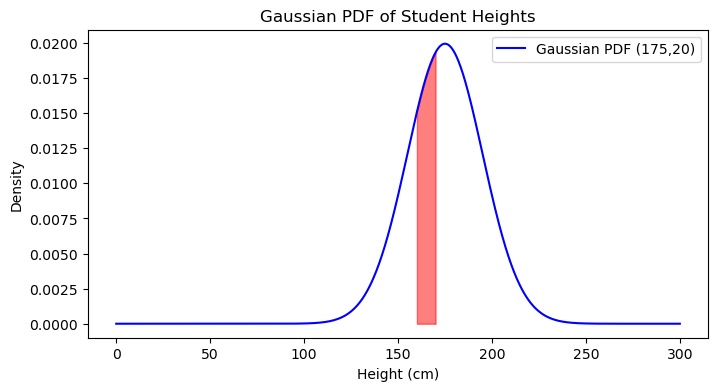
\includegraphics[scale=0.5]{Figures/GaussianPDF_height.png}
\end{figure} 
\end{frame} 


\begin{frame}{\textbf{Using PDF }}
The probability that a random variable M is between $a$ and $b$ is the area under the curve between $a$ and $b$. 
\[
P(0 \leq X \leq 300) = \int_{0}^{300} p(x) \, dx = 1
\]
 \begin{figure}
\centering
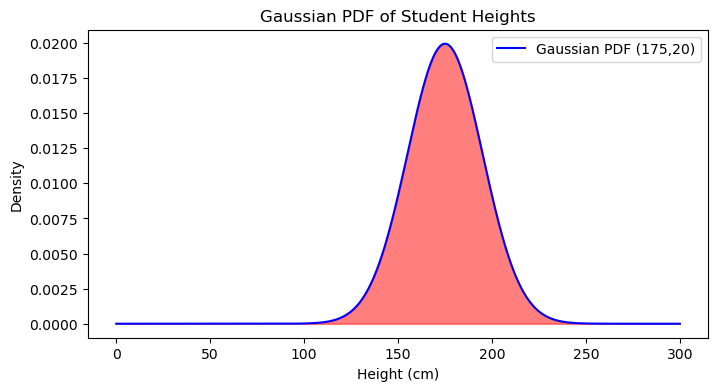
\includegraphics[scale=0.5]{Figures/GaussianPDF_height_all.png}
\end{figure} 
\end{frame} 


\begin{frame}{\textbf{Sampling from a Probability Distributions}}
 Drawing a sample from a probability distribution means selecting a value (or a set of values) according to the probability characteristics defined by that distribution. Essentially, it's a way of generating random numbers where the likelihood of each number being chosen is determined by the distribution's properties.

\begin{block}{Examples}
\begin{itemize}
  \item [$\bullet$] \textbf{Normal (Gaussian) Distribution:} Most samples will cluster around the mean, with the frequency of occurrence decreasing as you move away from the mean, following the bell curve shape.
  \item [$\bullet$] \textbf{Uniform Distribution:} Every number within a specified range has an equal chance of being selected.
\end{itemize}
\end{block}

\end{frame}


\begin{frame}{\textbf{Sampling from Gaussian vs Uniform PDF}}
If you draw 1000 samples 
 \begin{figure}
\centering
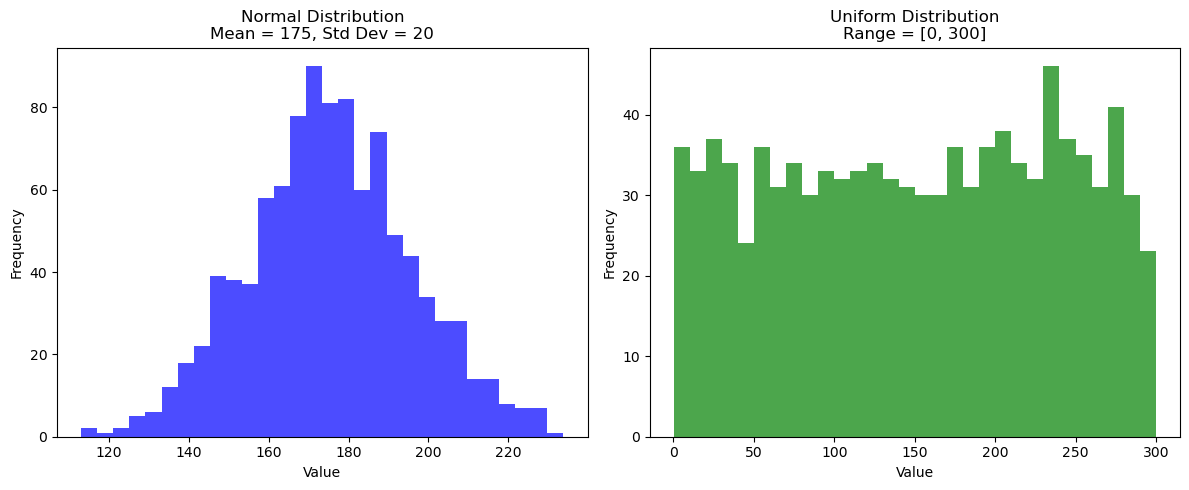
\includegraphics[scale=0.45]{Figures/sample_a_PDF.png}
\end{figure} 
\end{frame}


\begin{frame}{\textbf{Joint PDF and Marginal PDF}}
 \begin{figure}
\centering
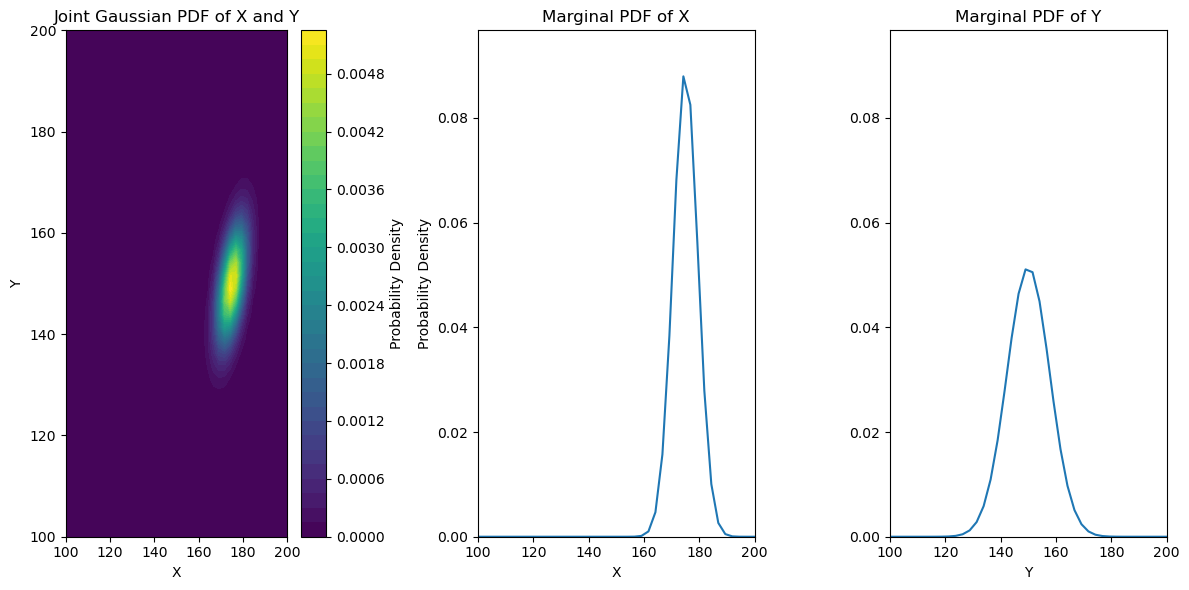
\includegraphics[scale=0.45]{Figures/joint_marginal.png}
\end{figure} 
\end{frame}





\begin{frame}{\textbf{Joint PDF - Independent vs Dependent Variables}}
Mathematical details are in the lecture script section 1.3 
 \begin{figure}
\centering
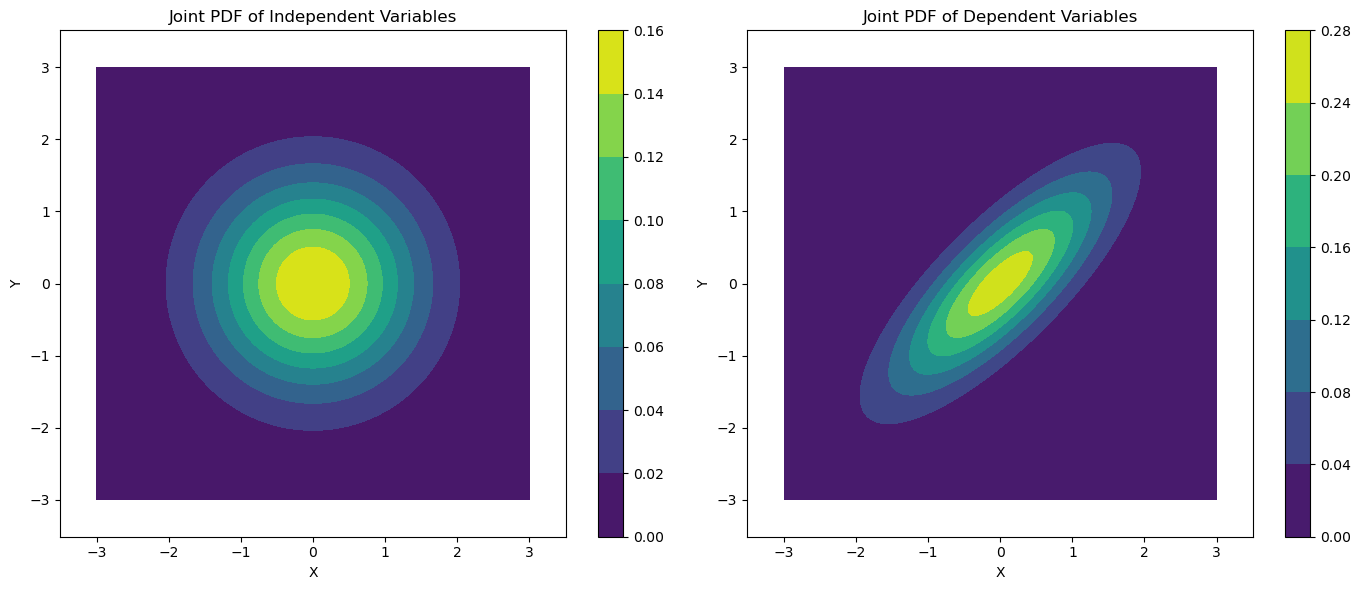
\includegraphics[scale=0.42]{Figures/joint_PDF_dependent_vs_independent.png}
\end{figure} 
\end{frame}

\begin{frame}{\textbf{Conditional Probability}}
Let's assume two vectors of random variables $\mathbf{x}$ and $\mathbf{y}$ such that their joint PDF is given by $p(\mathbf{x},\mathbf{y})$. The marginal PDF of $\mathbf{x}$ can be written as

\[ p(\mathbf{x}) = \int d\mathbf{y} \, p(\mathbf{x}, \mathbf{y}), \]
The conditional PDF $p(\mathbf{x}| \mathbf{y})$, i.e., the PDF of $\mathbf{x}$ given the values of $\mathbf{y}$, is defined as

\[ p(\mathbf{x}| \mathbf{y}) = \frac{p(\mathbf{x}, \mathbf{y})}{p(\mathbf{y})} \]

\[ p(\mathbf{y}| \mathbf{x}) = \frac{p(\mathbf{x}, \mathbf{y})}{p(\mathbf{x})} \]

\[ p(\mathbf{x}| \mathbf{y}) {p(\mathbf{y})} =  p(\mathbf{x}| \mathbf{y}) {p(\mathbf{y})} \] 
\end{frame}


\section{Bayes' Rule}
\subsection{}
\begin{frame}{\textbf{Bayes' Rule}} 

\[ p(\mathbf{x}| \mathbf{y}) = \frac{ p(\mathbf{y}| \mathbf{x}) p(\mathbf{x})}{p(\mathbf{y})}  \]

\begin{itemize}
  \item [$-$] $p(\mathbf{x} | \mathbf{y})$ is the \textbf{posterior probability distribution PPD} of vector $\mathbf{x}$ given vector $\mathbf{y}$.
  \item [$-$] $p(\mathbf{y} | \mathbf{x})$ is the \textbf{likelihood}, which is the probability distribution of observing vector $\mathbf{y}$ given vector $\mathbf{x}$.
  \item [$-$] $p(\mathbf{x})$ is the \textbf{prior} of vector $\mathbf{x}$, reflecting our beliefs about $\mathbf{x}$ before observing $\mathbf{y}$.
  \item [$-$] $p(\mathbf{y})$ is the evidence or \textbf{marginal PDF}, which normalizes the result. It is the overall probability of observing $\mathbf{y}$ under all possible $\mathbf{x}$ values and is computed as:
  \[
    p(\mathbf{y}) = \int p(\mathbf{y} | \mathbf{x}) \cdot p(\mathbf{x}) \, d\mathbf{x} \] 
  This integral sums (or integrates) over all possible values of vector $\mathbf{x}$.
\end{itemize}

\end{frame}



\begin{frame}{\textbf{Bayes' Rule}} 
\[ p(\mathbf{m}| \mathbf{d}) = \frac{ p(\mathbf{d}| \mathbf{m}) p(\mathbf{m})}{p(\mathbf{d})}  \]

\begin{itemize}
  \item [$-$] $p(\mathbf{m} | \mathbf{d})$ is the \textbf{posterior probability distribution PPD} of vector $\mathbf{m}$ given vector $\mathbf{d}$.
\end{itemize}
\end{frame}


\begin{frame}{\textbf{Bayes' Rule}} 

\[ p(\mathbf{m}| \mathbf{d}) = \frac{ p(\mathbf{d}| \mathbf{m}) p(\mathbf{m})}{p(\mathbf{d})}  \]

\begin{itemize}
  \item [$-$] $p(\mathbf{d} | \mathbf{m})$  is the \textbf{likelihood}, which is the probability distribution of observing vector $\mathbf{d}$ given vector $\mathbf{m}$
  \item [$-$] It shows how likely the model $\mathbf{m}$ produces the observed data $\mathbf{d}$
\end{itemize}
Assuming the data has Gaussian noise
\[
p(\mathbf{d} | \mathbf{m}) = \left((2\pi)^N |\mathbf{C}_{\mathbf{d}}|\right)^{-\frac{1}{2}}
\exp\left[ -\frac{1}{2} (\mathbf{d} - \mathbf{g}(\mathbf{m}))^\text{T} \mathbf{C}_{\mathbf{d}}^{-1} (\mathbf{d} - \mathbf{g}(\mathbf{m})) \right]
\]

\end{frame}


\begin{frame}{\textbf{Bayes' Rule}} 
\[ p(\mathbf{m}| \mathbf{d}) = \frac{ p(\mathbf{d}| \mathbf{m}) p(\mathbf{m})}{p(\mathbf{d})}  \]

\begin{itemize}
  \item [$-$] $p(\mathbf{m})$ is the \textbf{prior} of vector $\mathbf{m}$, reflecting our beliefs about $\mathbf{m}$ before observing $\mathbf{d}$.
  \item [$-$] If we have no idea about some possible $\mathbf{m}$ then it is desirable to draw the prior from uniform distribution.
  \item [$-$] If we believe that the model should be somewhere around $<\mathbf{m}>$ then we can draw prior from 
 \[
f(\mathbf{m}) = \left((2\pi)^M |\mathbf{C}_{\mathbf{m}}|\right)^{-\frac{1}{2}} 
\exp\left[ -\frac{1}{2} (\mathbf{m} - \langle\mathbf{m}\rangle)^\text{T} \mathbf{C}_{\mathbf{m}}^{-1} (\mathbf{m} - \langle\mathbf{m}\rangle) \right]
\] 

\[
p(\mathbf{d}|\mathbf{m}) = \frac{1}{[2\pi]^{N/2}} \exp\left[ -\frac{\chi^2}{2} \right], 
\]
\item $p(\mathbf{d})$ is a normalization constant, marginal PDF of data
\end{itemize}
\end{frame} 



\begin{frame}{\textbf{Bayes' Rule}}

\begin{itemize}
  \item[$\bullet$] How to compute \( p(\mathbf{m}|\mathbf{d}) \)?
  \item[$\bullet$] If all distributions involved (\( p(\mathbf{m}) \), \( p(\mathbf{d}|\mathbf{m}) \) and \( p(\mathbf{d}) \)) are analytically describable (including the likelihood), we can for some cases find analytical descriptions of \( p(\mathbf{m}|\mathbf{d}) \). This is in fact what we did all the time when we considered linear inversion!
  \item[$\bullet$] If the problem is low dimensional and if the forward problem is fast to solve, we can evaluate \( p(\mathbf{m}) \), \( p(\mathbf{d}|\mathbf{m}) \) and \( p(\mathbf{d}) \) over a large grid and calculate. This is called grid search.
  \item[$\bullet$] In high dimensions, this will not work anymore.
\end{itemize}

\end{frame}

\section{Bayesian Inversion}
\subsection{}

\begin{frame}
\frametitle{\textbf{Grid Search Algorithm for Bayesian Inversion}}
\footnotesize
Define grid over parameter space of model $\mathbf{m}$ \\
\textcolor{blue}{Loop over grid points}\\
\hspace{1cm} Compute likelihood \( p(\mathbf{d}|\mathbf{m}_i) \) using forward model \vspace{0.1cm}\\
\hspace{1cm} Compute prior probability \( p(\mathbf{m}_i) \) \vspace{0.1cm}\\
\hspace{1cm} Unnormalized posterior at grid point $i$: \( p(\mathbf{m}_i|\mathbf{d}) \propto p(\mathbf{d}|\mathbf{m}_i) \times p(\mathbf{m}_i) \) \vspace{0.1cm}\\
\textcolor{cyan}{end Loop}\\
Compute marginal likelihood \( p(\mathbf{d}) \approx \sum_i p(\mathbf{d}|\mathbf{m}_i) \times p(\mathbf{m}_i) \) \\
\textcolor{blue}{Loop over grid points again}\\
\hspace{1cm} Normalize posterior: \( p(\mathbf{m}_i|\mathbf{d}) = \frac{p(\mathbf{d}|\mathbf{m}_i) \times p(\mathbf{m}_i)}{p(\mathbf{d})} \) \vspace{0.1cm}\\
\textcolor{cyan}{end Loop}\\
\textbf{Output:} Estimated posterior probability distribution \( p(\mathbf{m}|\mathbf{d}) \)\\
\end{frame}


\begin{frame}
\frametitle{\textbf{Monte Carlo Algorithm for Bayesian Inversion}}
\footnotesize
\textcolor{blue}{Define the prior distribution for model parameters $\mathbf{m}$} \\
\textcolor{blue}{Sample a large number of parameter sets $\{\mathbf{m}_i\}$ from the prior distribution} \\
\textcolor{blue}{Loop over Monte Carlo samples} \\
\hspace{1cm} For each sample $\mathbf{m}_i$: \\
\hspace{1cm} Compute likelihood \( p(\mathbf{d}|\mathbf{m}_i) \) using forward model \vspace{0.1cm} \\
\hspace{1cm} Unnormalized posterior: \( p(\mathbf{m}_i|\mathbf{d}) \propto p(\mathbf{d}|\mathbf{m}_i) \times p(\mathbf{m}_i) \) \vspace{0.1cm} \\
\textcolor{cyan}{end Loop} \\
\textcolor{blue}{Compute the normalization constant (marginal likelihood)} \\
\hspace{1cm} \( p(\mathbf{d}) \approx \frac{1}{N} \sum_i p(\mathbf{d}|\mathbf{m}_i) \times p(\mathbf{m}_i) \) where $N$ is the number of samples \vspace{0.1cm} \\
\textcolor{blue}{Normalize the posterior distribution} \\
\hspace{1cm} Normalize each unnormalized posterior: \( p(\mathbf{m}_i|\mathbf{d}) = \frac{p(\mathbf{m}_i|\mathbf{d})}{\sum_j p(\mathbf{m}_j|\mathbf{d})} \) \vspace{0.1cm} \\
\textbf{Output:} Estimated posterior probability distribution \( p(\mathbf{m}|\mathbf{d}) \) based on Monte Carlo samples\\
\end{frame}




\section{Markov Chain}
\subsection{}

\begin{frame}
\frametitle{Introduction to Markov Chain}
\begin{itemize}
    \item A Markov chain is a stochastic process with the Markov property of memorylessness.
    \item We will consider a simple weather model as an example.
    \item The states are Sunny (S), Cloudy (C), and Rainy (R).
\end{itemize}
\end{frame}

\begin{frame}
\frametitle{Transition Matrix}
The transition probabilities between different weather states are given by:
\[
\begin{bmatrix}
0.7 & 0.2 & 0.1 \\
0.3 & 0.4 & 0.3 \\
0.2 & 0.3 & 0.5 \\
\end{bmatrix}
\]
\begin{itemize}
    \item From \textbf{Sunny}, the next day has:
    \begin{itemize}
        \item 70\% chance of being Sunny
        \item 20\% chance of being Cloudy
        \item 10\% chance of being Rainy
    \end{itemize}
    \item From \textbf{Cloudy}, the next day has:
    \begin{itemize}
        \item 30\% chance of being Sunny
        \item 40\% chance of being Cloudy
        \item 30\% chance of being Rainy
    \end{itemize}
    \item From \textbf{Rainy}, the next day has:
    \begin{itemize}
        \item 20\% chance of being Sunny
        \item 30\% chance of being Cloudy
        \item 50\% chance of being Rainy
    \end{itemize}
\end{itemize}
\end{frame}

\begin{frame}
\frametitle{Irreducibility and Ergodicity}
\begin{itemize}
    \item \textbf{Irreducibility}: It is possible to reach any state from any state.
    \item \textbf{Ergodicity}: Long-term average behavior converges to a stationary distribution regardless of the initial state.
\end{itemize}
\end{frame}

\begin{frame}
\LARGE Verify the Irreucibility and Ergodicity with an example 
    
\end{frame}

\begin{frame}
\frametitle{How to we generate proposal models?}

\begin{itemize}
  \item \textbf{Gaussian Distribution}
  \begin{itemize}
    \item Symmetric Gaussian: Centered at the current state with fixed variance.
    \item Adaptive Gaussian: Variance adjusted based on sampling dynamics.
  \end{itemize}

  \item \textbf{Random Walk Proposals}
  Random walk proposals are a popular choice in the Metropolis-Hastings algorithm, particularly when the form of the target distribution is complex or unknown.  The idea is to generate a new sample by slightly modifying the current sample, using a stochastic rule.

  \item \textbf{Laplace Distribution}
  \begin{itemize}
    \item Similar to Gaussian but with sharper peaks and heavier tails, enhancing exploration.
  \end{itemize}

  \item \textbf{Multimodal Proposals}
  \begin{itemize}
    \item Designed to propose states across different modes in a multimodal distribution.
  \end{itemize}

  \item \textbf{Proposal from Prior}
  \begin{itemize}
    \item Sampling directly from the prior distribution, especially when the prior is informative.
  \end{itemize}
\end{itemize}

\end{frame} 


\section{MCMC}
\subsection{}

\begin{frame}{\textbf{MCMC Algorithm - Metropolis-Hasting}}
    \begin{enumerate}
        \item \textbf{Initialization:}
        \begin{itemize}
            \item Initialize model parameters $\mathbf{m}_0$.
            \item Choose a proposal distribution $q(\mathbf{m}'|\mathbf{m})$.
            \item Define number of iterations $N$.
        \end{itemize}
        
        \item \textbf{Iteration} (for $i = 1$ to $N$):
        \begin{itemize}
            \item \textbf{Generate Proposal:}
            \begin{itemize}
                \item Draw candidate model $\mathbf{m}'$ from $q(\mathbf{m}'|\mathbf{m}_{i-1})$.
            \end{itemize}
            \item \textbf{Calculate Acceptance Probability} $\alpha$:
            \begin{itemize}
                \item Compute likelihoods and priors.
                \item $\alpha = \min \left(1, \frac{p(\mathbf{d}|\mathbf{m}') p(\mathbf{m}') q(\mathbf{m}_{i-1}|\mathbf{m}')}{p(\mathbf{d}|\mathbf{m}_{i-1}) p(\mathbf{m}_{i-1}) q(\mathbf{m}'|\mathbf{m}_{i-1})} \right)$.
            \end{itemize}
            \item \textbf{Accept or Reject:}
            \begin{itemize}
                \item Draw $u \sim U(0, 1)$.
                \item If $u \leq \alpha$, set $\mathbf{m}_i = \mathbf{m}'$; otherwise $\mathbf{m}_i = \mathbf{m}_{i-1}$.
            \end{itemize}
        \end{itemize}
        
        \item \textbf{Output:}
        \begin{itemize}
            \item Return the chain $\{\mathbf{m}_1, \mathbf{m}_2, \ldots, \mathbf{m}_N\}$.
        \end{itemize}
    \end{enumerate}
\end{frame}


\begin{frame}{\textbf{MCMC-Metropolis Hasting - Log Likelihood}}
    \begin{enumerate}
        \item \textbf{Initialization:}
        \begin{itemize}
            \item Initialize model parameters $\mathbf{m}_0$.
            \item Choose a proposal distribution $q(\mathbf{m}'|\mathbf{m})$.
            \item Define number of iterations $N$.
        \end{itemize}
        
        \item \textbf{Iteration} (for $i = 1$ to $N$):
        \begin{itemize}
            \item \textbf{Generate Proposal:}
            \begin{itemize}
                \item Draw candidate model $\mathbf{m}'$ from $q(\mathbf{m}'|\mathbf{m}_{i-1})$.
            \end{itemize}
            \item \textbf{Calculate Acceptance Probability} $\alpha$ using log likelihood:
            \begin{itemize}
                \item Compute $\text{log\_alpha} = \left( \log p(\mathbf{d}|\mathbf{m}') + \log p(\mathbf{m}') + \log q(\mathbf{m}_{i-1}|\mathbf{m}') \right) - \left( \log p(\mathbf{d}|\mathbf{m}_{i-1}) + \log p(\mathbf{m}_{i-1}) + \log q(\mathbf{m}'|\mathbf{m}_{i-1}) \right)$.
                \item $\alpha = \min \left(1, \exp(\text{log\_alpha}) \right)$.
            \end{itemize}
            \item \textbf{Accept or Reject:}
            \begin{itemize}
                \item Draw $u \sim U(0, 1)$.
                \item If $u \leq \alpha$, set $\mathbf{m}_i = \mathbf{m}'$; otherwise $\mathbf{m}_i = \mathbf{m}_{i-1}$.
            \end{itemize}
        \end{itemize}
        
        \item \textbf{Output:}
        \begin{itemize}
            \item Return the chain $\{\mathbf{m}_1, \mathbf{m}_2, \ldots, \mathbf{m}_N\}$.
        \end{itemize}
    \end{enumerate}
\end{frame}



\begin{frame}\frametitle{Variants of MCMC Algorithms}

\begin{itemize}
    \item \textbf{Metropolis-Hastings (MH) Algorithm}: Basic method using proposal distributions and acceptance probability.
    
    \item \textbf{Gibbs Sampling}: Samples from conditionals, suitable for decomposable joint distributions.
    
    \item \textbf{Hamiltonian Monte Carlo (HMC)}: Efficiently proposes samples by simulating trajectories in position and momentum space.
    
    \item \textbf{Slice Sampling}: Constructs slices around states for uniform sampling, useful for conditional distributions.
    
    \item \textbf{Parallel Tempering (PT)}: Employs multiple chains at different "temperatures" for exploring multimodal distributions.
    
    \item \textbf{Adaptive MCMC}: Adjusts proposal distribution or parameters to improve efficiency.
    
    \item \textbf{Sequential Monte Carlo (SMC)}: Combines importance sampling and resampling for sampling sequences of distributions.
    
    \item \textbf{Reversible-Jump Hamiltonian Monte Carlo (RJHMC)}: Extends HMC to handle varying dimensionality of parameter space.
\end{itemize}

\end{frame}


%000000000
\begin{frame}
\frametitle{\textbf{Hamiltomian MC (HMC)}}



$H(\mathbf{m}, \mathbf{p}) = U(\mathbf{m}) + K(\mathbf{p})$

\begin{itemize}
    \item \( U(\mathbf{m}) \): Potential energy (negative log-likelihood).
    \item \( K(\mathbf{p}) \): Kinetic energy, \( K(\mathbf{p}) = \frac{1}{2} \mathbf{p}^T \mathbf{M}^{-1} \mathbf{p} \).
\end{itemize}

\begin{enumerate}
    \item [-] \textbf{Momentum Half-Step:}
    \[
    \mathbf{p}_{t + \epsilon/2} = \mathbf{p}_t - \frac{\epsilon}{2} \nabla U(\mathbf{m}_t)
    \]
    \item [-] \textbf{Position Full Step:}
    \[
    \mathbf{m}_{t + \epsilon} = \mathbf{m}_t + \epsilon \mathbf{M}^{-1} \mathbf{p}_{t + \epsilon/2}
    \]
    \item [-] \textbf{Momentum Half-Step Completion:}
    \[
    \mathbf{p}_{t + \epsilon} = \mathbf{p}_{t + \epsilon/2} - \frac{\epsilon}{2} \nabla U(\mathbf{m}_{t + \epsilon})
    \]
\end{enumerate}
After several iterations, \( \mathbf{m}_{t + \epsilon} \) and \( \mathbf{p}_{t + \epsilon} \) propose the new states \( \mathbf{m}' \) and \( \mathbf{p}' \).

\end{frame}

\begin{frame}{HMC}
\begin{block}{Algorithm Steps}
\begin{enumerate}
    \item \textbf{Initialization:}
    \begin{itemize}
        \item Initialize the parameter vector \( \mathbf{m}_0 \) and choose an initial momentum \( \mathbf{p}_0 \) from a typical distribution, e.g., \( N(0, \mathbf{I}) \).
    \end{itemize}
    
    \item \textbf{For each iteration \( i \) from 1 to N:}
    \begin{enumerate}
        \item \textbf{Resample Momentum:} Draw \( \mathbf{p}_i \) from \( N(0, \mathbf{I}) \).
        \item \textbf{Simulate Hamiltonian Dynamics:} Use the leapfrog method to numerically integrate Hamilton's equations, proposing \( \mathbf{m}' \) and \( \mathbf{p}' \).
        \item \textbf{Metropolis Accept-reject}
        \begin{itemize}
            \item Calculate the acceptance probability:
            \[
            \alpha = \min\left(1, \exp(-H(\mathbf{m}', \mathbf{p}') + H(\mathbf{m}_i, \mathbf{p}_i))\right)
            \]
            \item Accept or reject \( (\mathbf{m}', \mathbf{p}') \) based on \( \alpha \).
        \end{itemize}
    \end{enumerate}
    
    \item \textbf{Output:} Collect the samples \( \{\mathbf{m}_1, \mathbf{m}_2, \ldots, \mathbf{m}_N\} \).
\end{enumerate}
\end{block}
\end{frame}



\begin{frame}{\textbf{(Transdimentional) Reversible-jump HMCMC} }

\[ p(k, \mathbf{m}|\mathbf{d}) = \frac{p(k) p(\mathbf{m}|k) p(\mathbf{d}|\mathbf{m},k)}{\sum_{k' \in \kappa} p(k') p(\mathbf{m}|k') p(\mathbf{d}|\mathbf{m},k') \, d\mathbf{m}} 
\]

\[
p(\mathbf{m}|k) = 
\begin{cases}
\frac{1}{\sqrt{v_{\text{max}} - v_{\text{min}}}} & \text{if } v_{\text{min}} \leq v \leq v_{\text{max}} \\
0 & \text{Otherwise.}
\end{cases}
\]

\[
p(\mathbf{d}|\mathbf{m}, k) = \frac{1}{[2\pi]^{N/2}} \exp\left[ -\frac{\chi^2}{2} \right], 
\]


\[
\alpha(\mathbf{k}', \mathbf{m}'|\mathbf{k}, \mathbf{m}) = \min \left[ 1, \frac{\pi(\mathbf{m}', \mathbf{k}') q(\mathbf{m}|\mathbf{k}')}{\pi(\mathbf{m}, \mathbf{k}) q(\mathbf{m}'|\mathbf{k})} |J| \right],
\]
\end{frame}

\section{Geophysical Examples}
\subsection{}

\begin{frame}{RJHMCMC}
Show the video on Powerpoint 
\begin{figure}
    \centering
    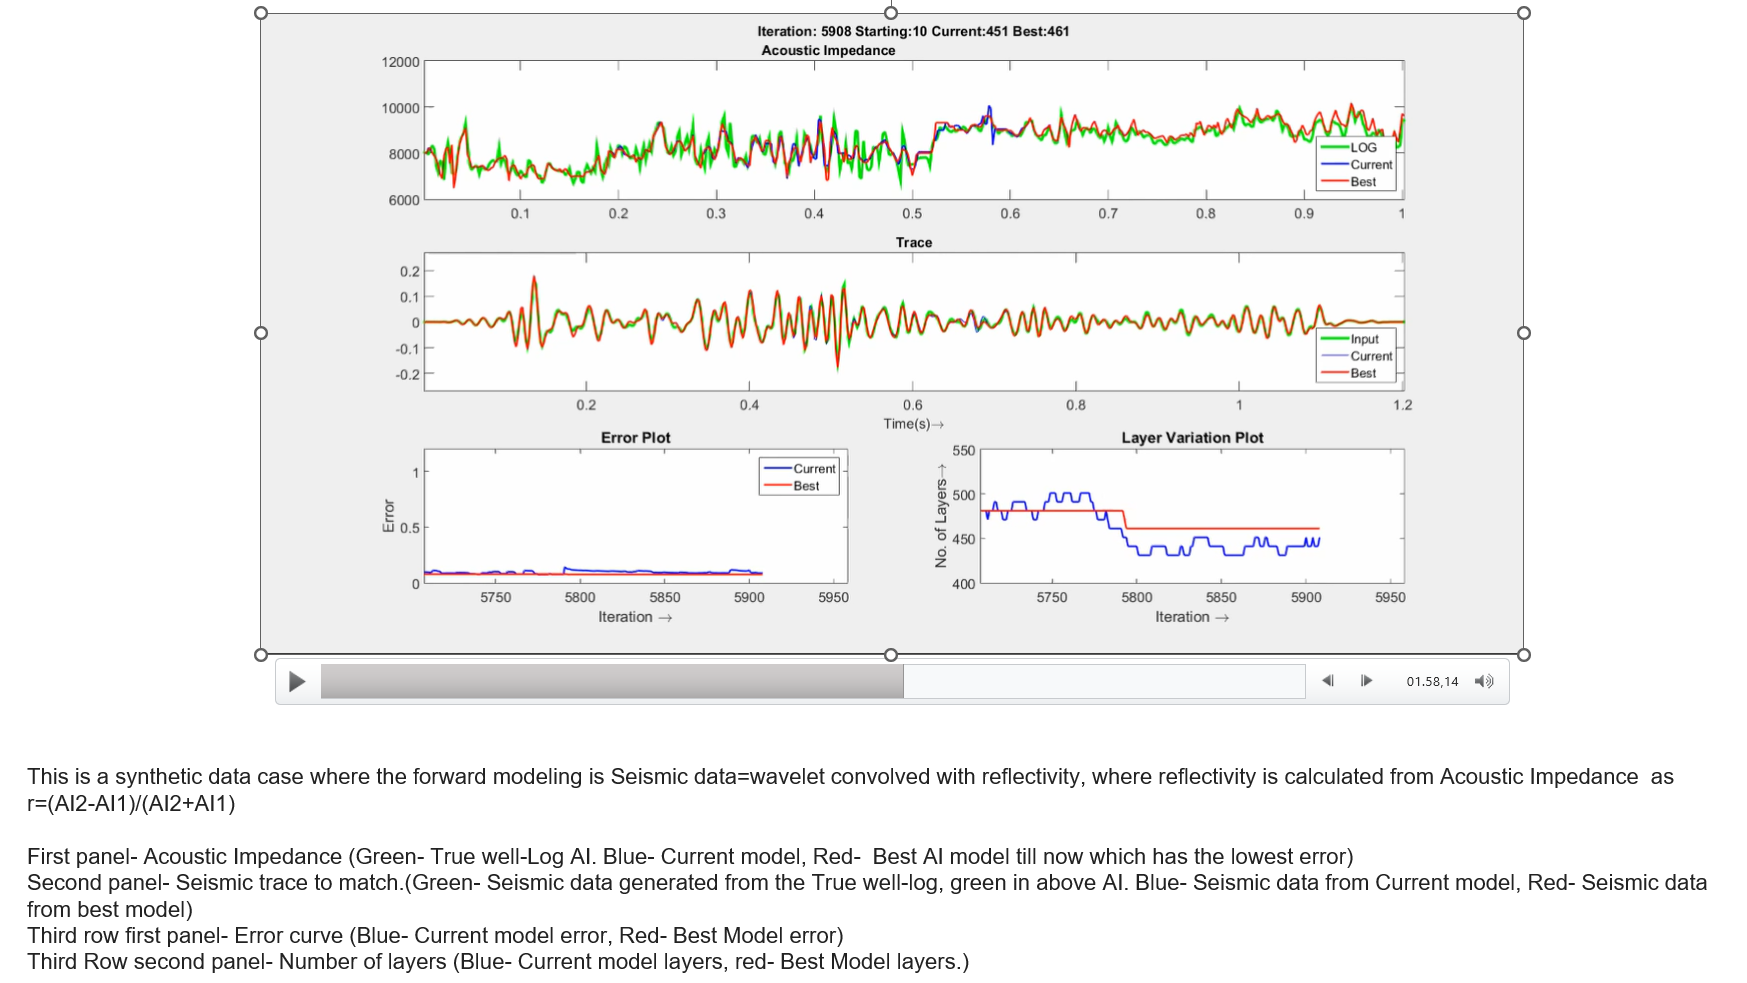
\includegraphics[scale=0.25]{Figures/RJHMCMC_seismictrace.PNG}
    \label{fig:enter-label}
    
    \small{Sen, Mrinal K., and Reetam Biswas. "Transdimensional seismic inversion using the reversible jump Hamiltonian Monte Carlo algorithm." Geophysics 82.3 (2017): R119-R134.}
\end{figure}
\end{frame}

\begin{frame}{\textbf{RJMCMC- 2D Seismic Inversion}}
\begin{figure}
    \centering
    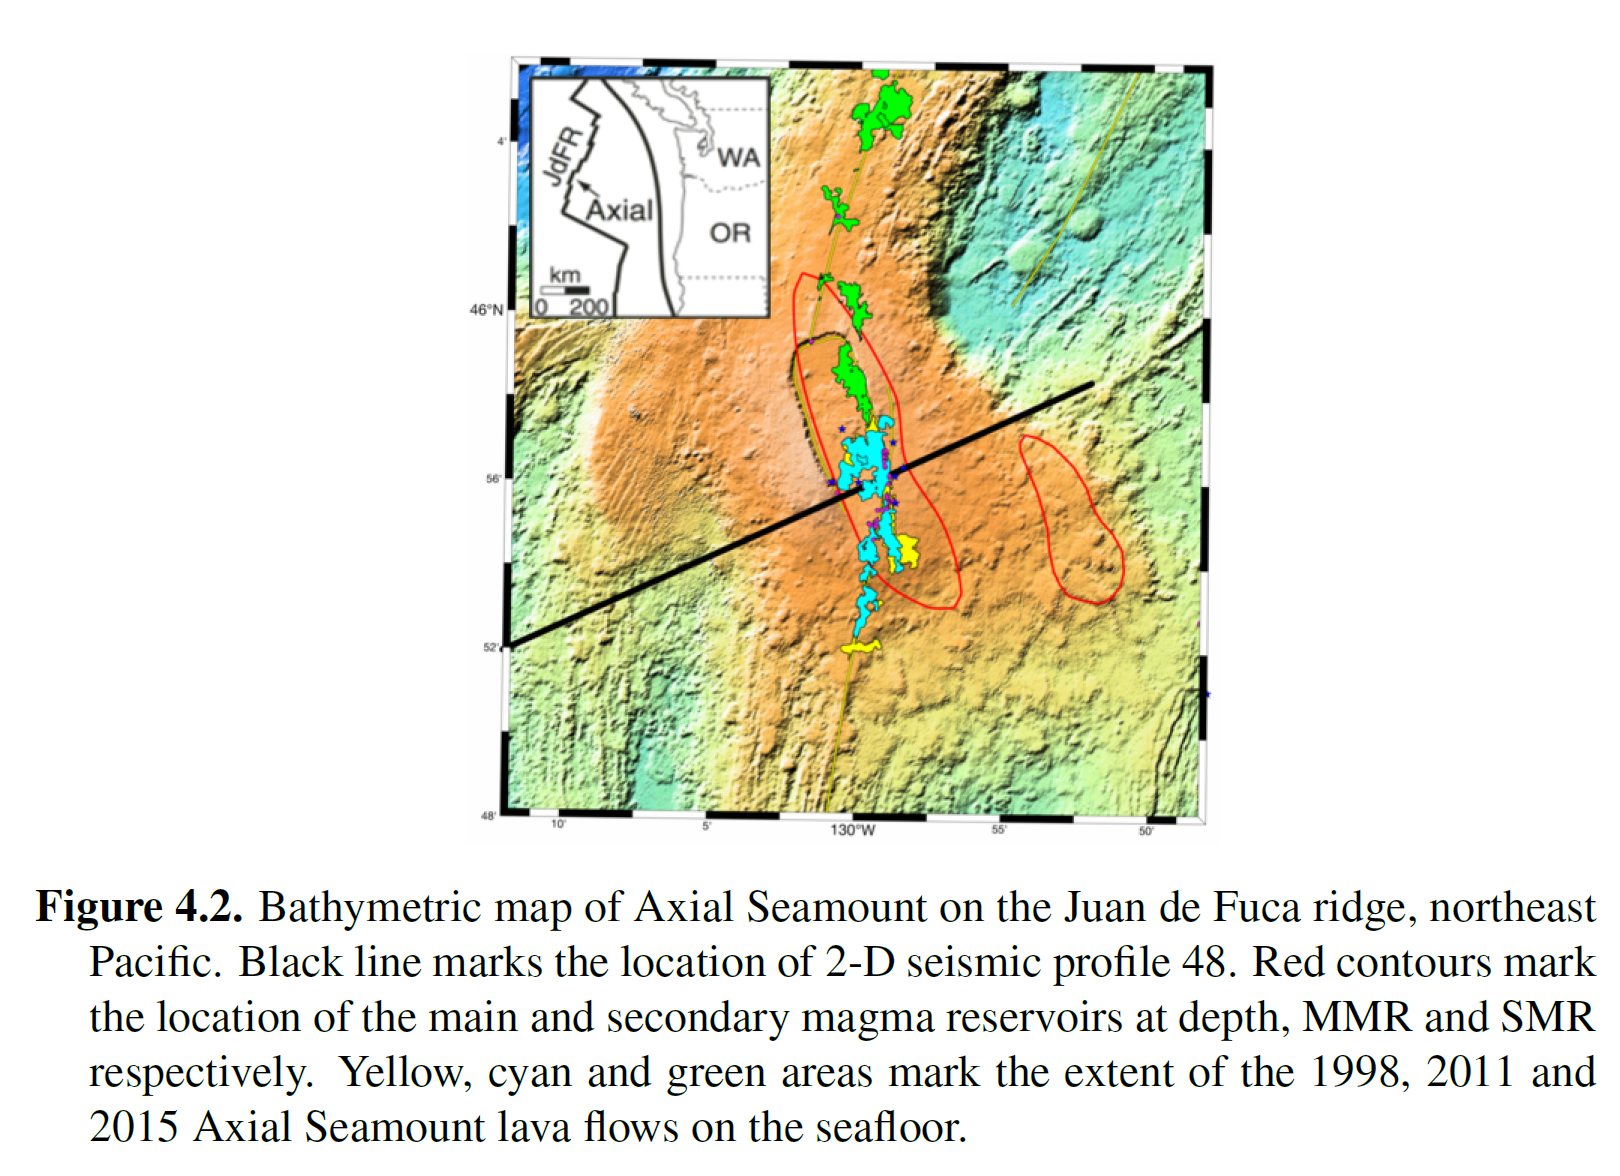
\includegraphics[scale=0.25]{Figures/axialseamount_topo.PNG}
    \label{fig:enter-label}
    
\tiny{Biswas, R., Arnulf, A. F., Sen, M. K., Datta, D., Zhao, Z., Mishra, P. K., Jaysaval, P. (2020, October). Two-step velocity inversion using trans-dimensional tomography and elastic FWI. In SEG International Exposition and Annual Meeting (p. D031S069R003). SEG.} 
\end{figure}   
\end{frame}

\begin{frame}{\textbf{RJMCMC- 2D Seismic Inversion}}
\begin{figure}
    \centering
    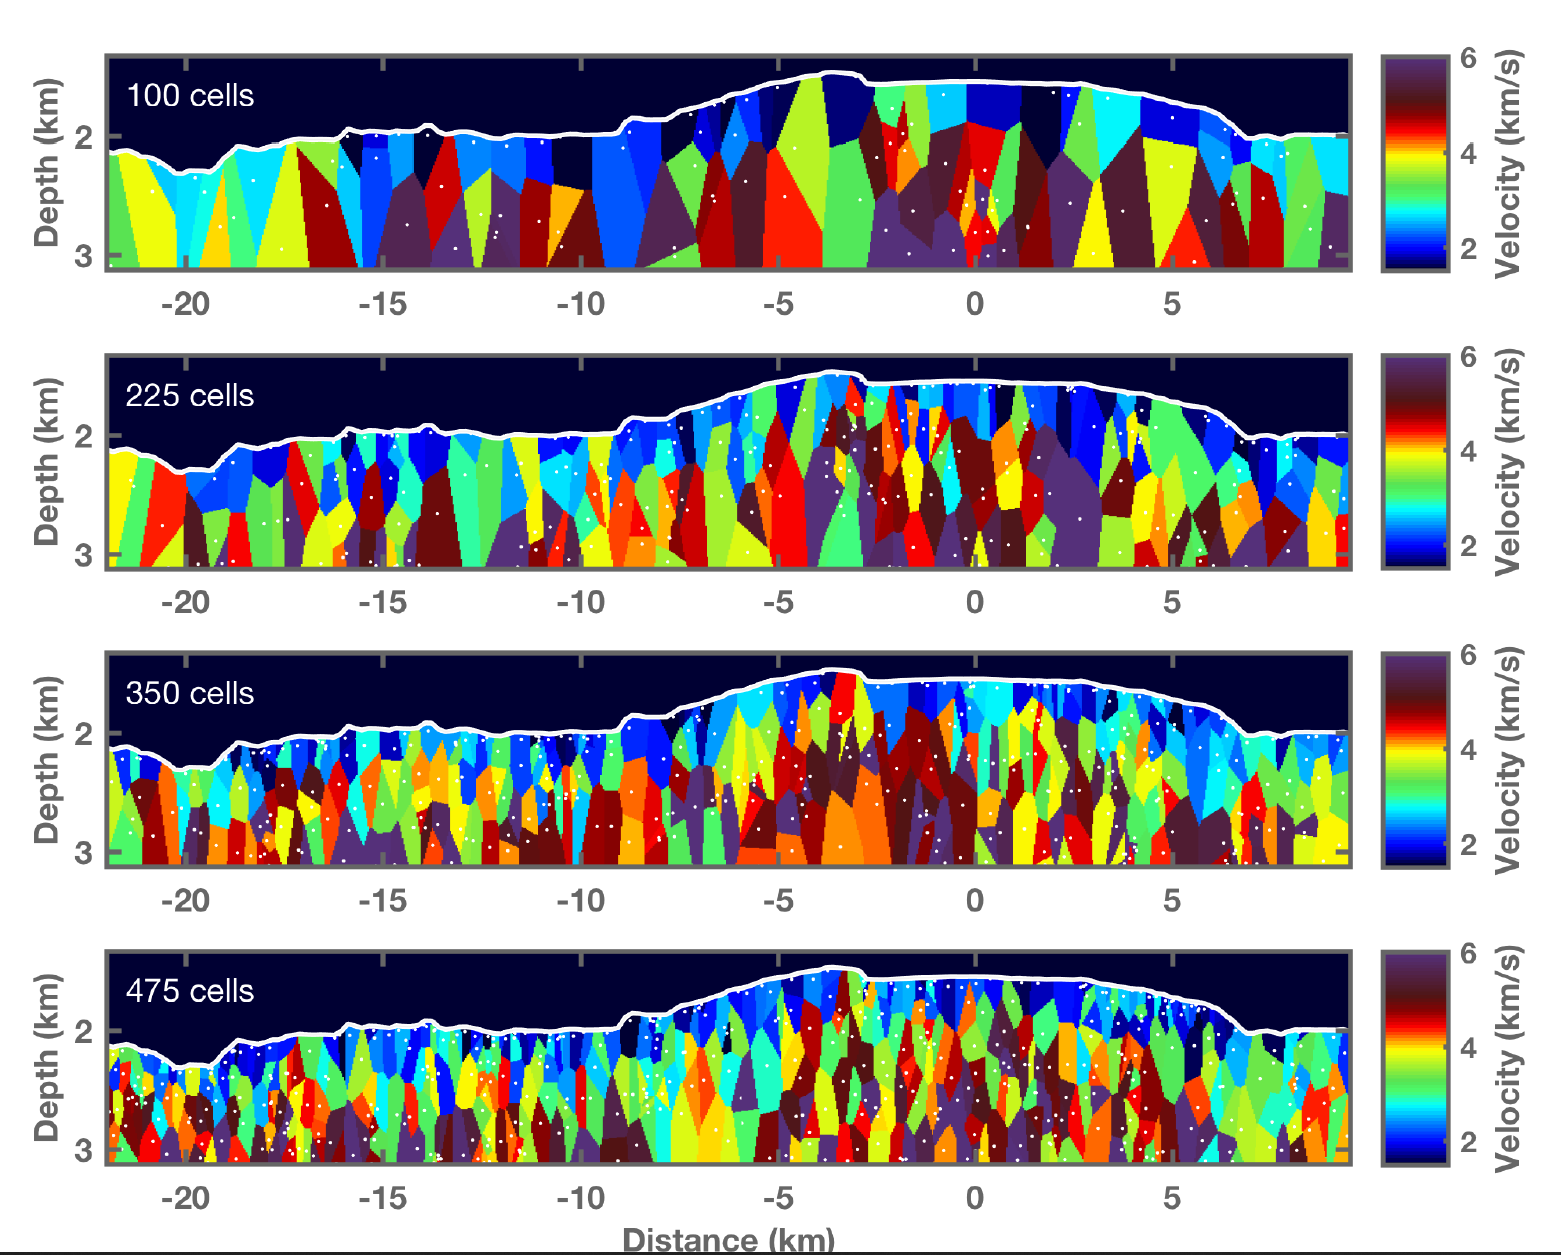
\includegraphics[scale=0.25]{Figures/axialseamount_voronoi.PNG}
    \label{fig:enter-label}
    
\tiny{Biswas, R., Arnulf, A. F., Sen, M. K., Datta, D., Zhao, Z., Mishra, P. K., Jaysaval, P. (2020, October). Two-step velocity inversion using trans-dimensional tomography and elastic FWI. In SEG International Exposition and Annual Meeting (p. D031S069R003). SEG.} 
\end{figure}   
\end{frame}

\begin{frame}{\textbf{RJMCMC- 2D Seismic Inversion}}
\begin{figure}
    \centering
    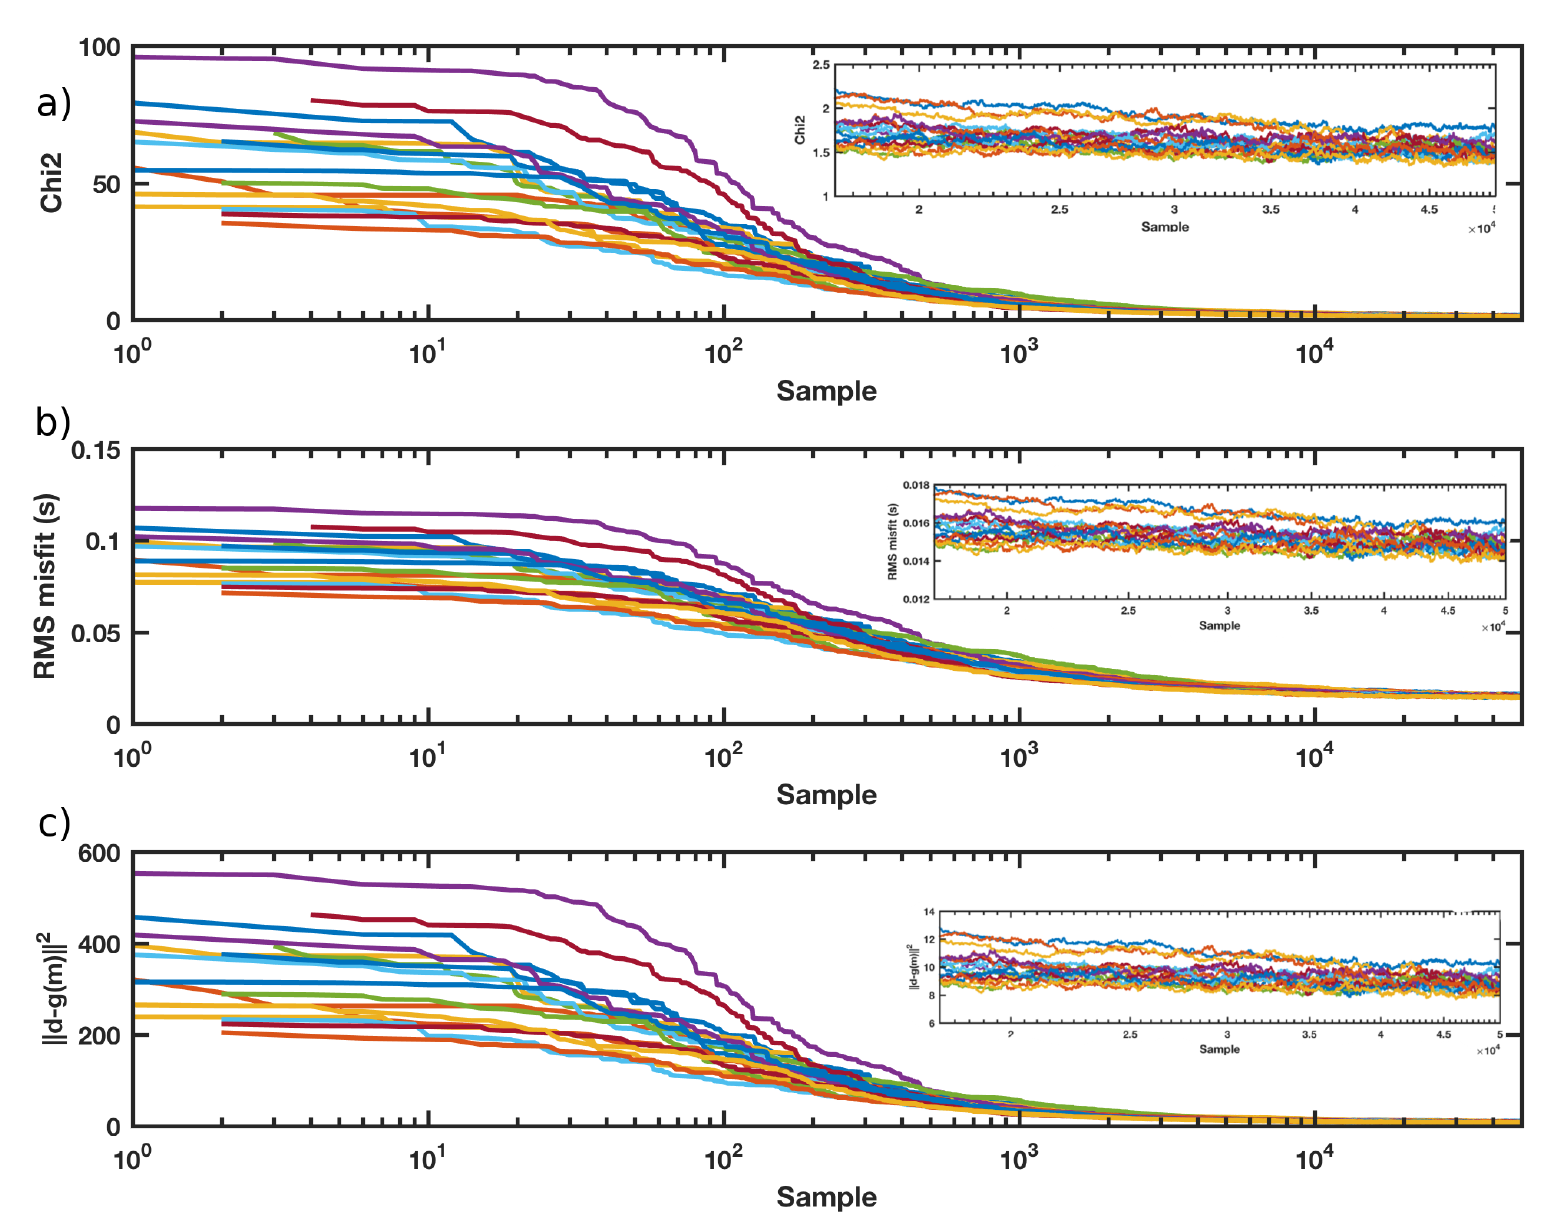
\includegraphics[scale=0.25]{Figures/axial_convergence.PNG}
    \label{fig:enter-label}
    
\tiny{Biswas, R., Arnulf, A. F., Sen, M. K., Datta, D., Zhao, Z., Mishra, P. K., Jaysaval, P. (2020, October). Two-step velocity inversion using trans-dimensional tomography and elastic FWI. In SEG International Exposition and Annual Meeting (p. D031S069R003). SEG.} 
\end{figure}   
\end{frame}

\begin{frame}{\textbf{RJMCMC- 2D Seismic Inversion}}
\begin{figure}
    \centering
    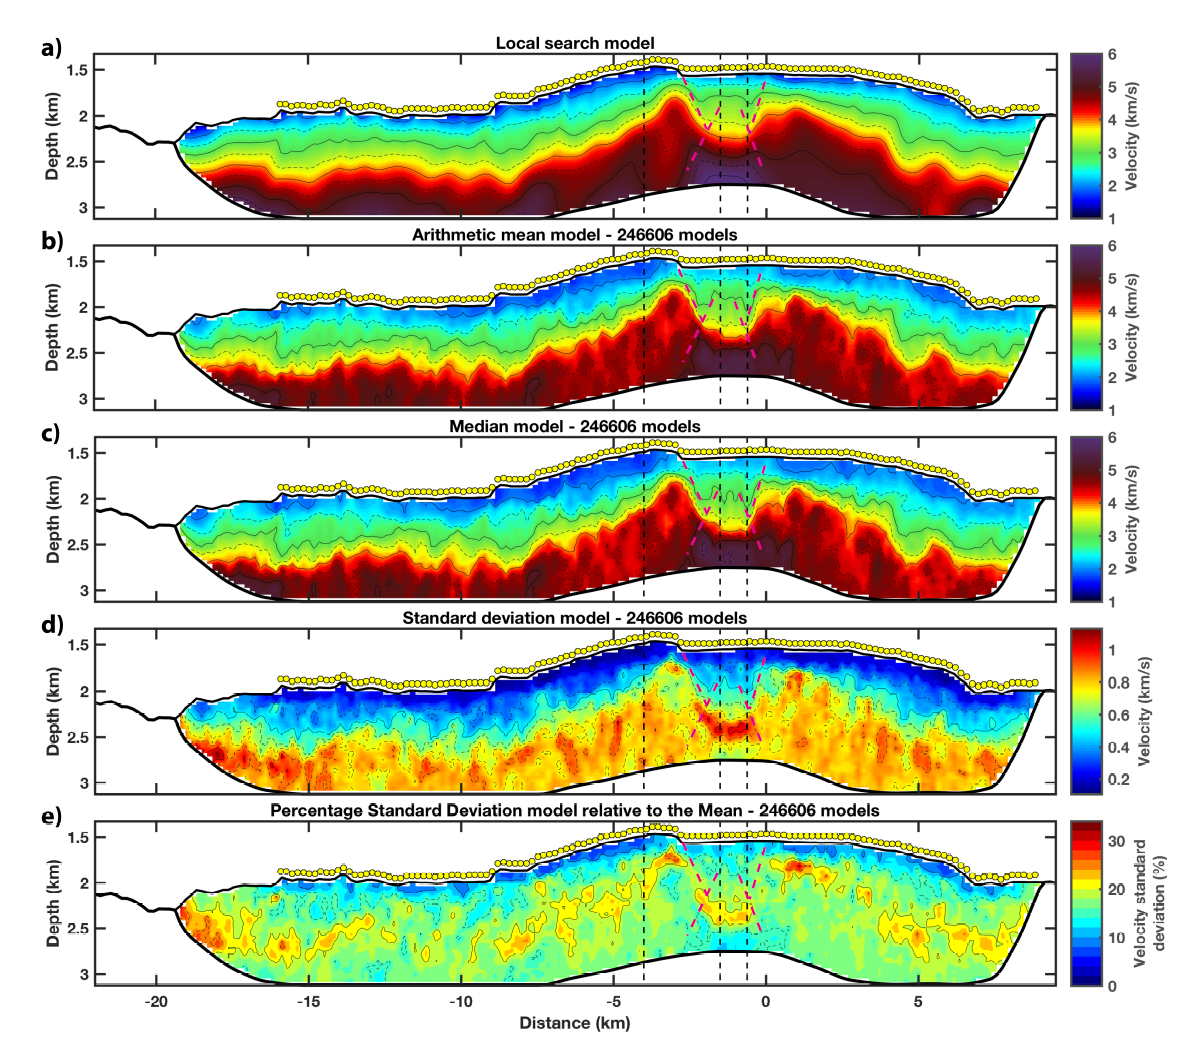
\includegraphics[scale=0.25]{Figures/axial_results.PNG}
    \label{fig:enter-label}
    
\tiny{Biswas, R., Arnulf, A. F., Sen, M. K., Datta, D., Zhao, Z., Mishra, P. K., Jaysaval, P. (2020, October). Two-step velocity inversion using trans-dimensional tomography and elastic FWI. In SEG International Exposition and Annual Meeting (p. D031S069R003). SEG.} 
\end{figure}   
\end{frame}

\begin{frame}{\textbf{RJMCMC- 2D Seismic Inversion}}
\begin{figure}
    \centering
    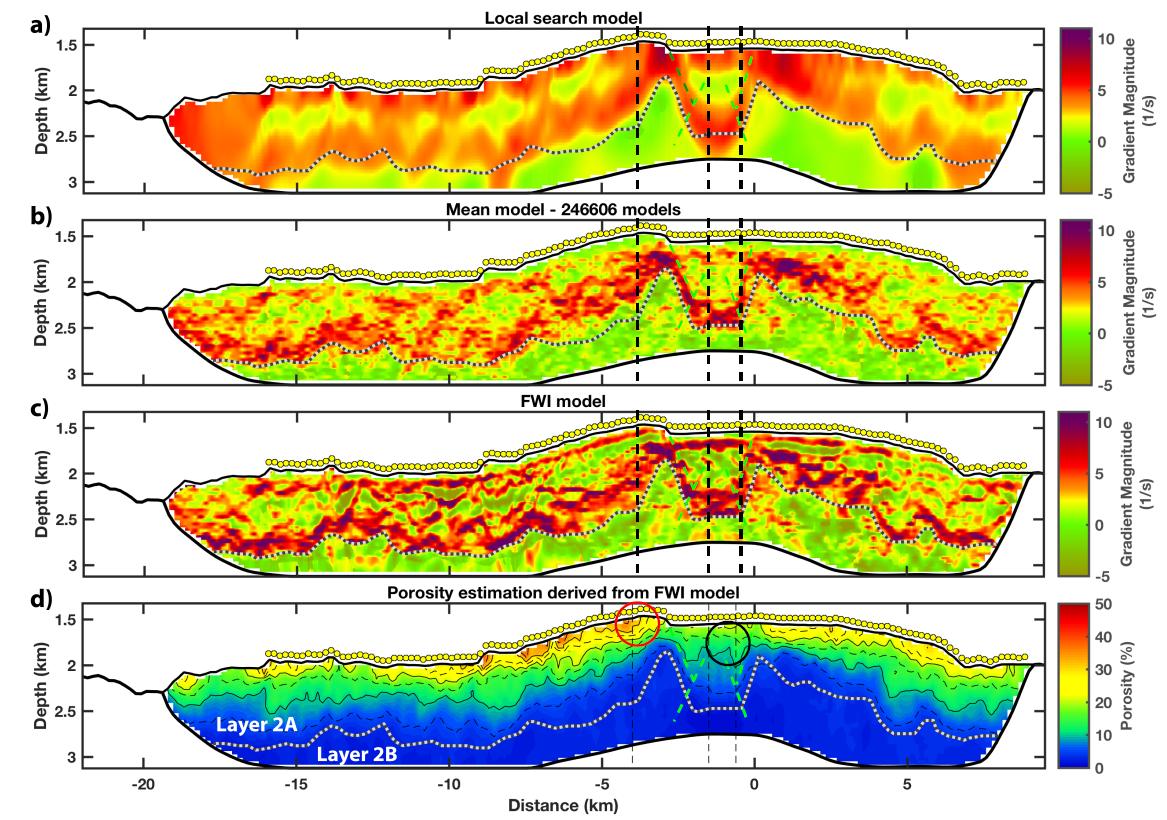
\includegraphics[scale=0.25]{Figures/axial_velocity_gradient.PNG}
    \label{fig:enter-label}
    
\tiny{Biswas, R., Arnulf, A. F., Sen, M. K., Datta, D., Zhao, Z., Mishra, P. K., Jaysaval, P. (2020, October). Two-step velocity inversion using trans-dimensional tomography and elastic FWI. In SEG International Exposition and Annual Meeting (p. D031S069R003). SEG.} 
\end{figure}   
\end{frame} 

\begin{frame}{\textbf{RJMCMC- 2D Seismic Inversion}}
\begin{figure}
    \centering
    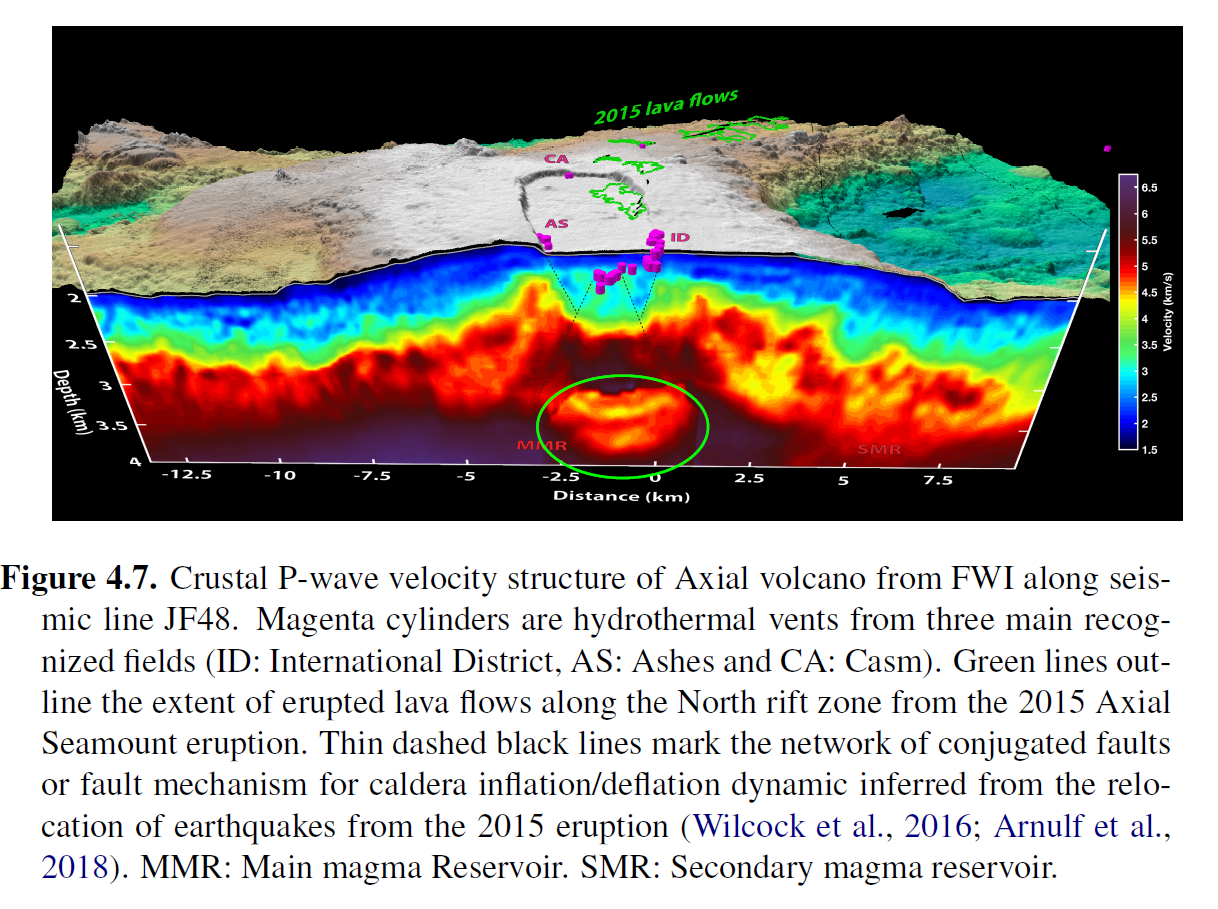
\includegraphics[scale=0.25]{Figures/axial_final.PNG}
    \label{fig:enter-label}
    
\tiny{Biswas, R., Arnulf, A. F., Sen, M. K., Datta, D., Zhao, Z., Mishra, P. K., Jaysaval, P. (2020, October). Two-step velocity inversion using trans-dimensional tomography and elastic FWI. In SEG International Exposition and Annual Meeting (p. D031S069R003). SEG.} 
\end{figure}   
\end{frame} 

\section{Future Directions} 
\subsection{}

\begin{frame}{\textbf{Future directions}}
\begin{itemize}
    \item [$\bullet$] For single domain geophysical inversion there seems to be sufficient number of algorithms to do the job.
    \item [$\bullet$] We need FAST! forward solvers. Can we train Deep Neural Networks to solve forward problems? Check out \textbf{NeuralOperators}, \textbf{DeepONet}. Research is in early phase. GTK has a project named \textbf{MULTIVERSE}. Check out \textbf{randomized linear algebra}, can do faster matrix operations 
    \item [$\bullet$] Can we use Neural network to propose models for stochastic inversion? Physics-based DNN for inverse problems. Check out {https://doi.org/10.1190/tle41060375.1} Also in GTK's \textbf{MULTIVERSE} 
    \item [$\bullet$] Multiphysics joint-inversion with Stochastic methods.
    \item [$\bullet$] With Tensorflow/Pytorch/Flux, we can use automatic differentiation for gradient computations. Also check out Machine learning methods for local optimisation: \textbf{Batch Gradient Descent}, \textbf{Mini-batch Gradient descent}, \textbf{DeepWave}.
    \item [$\bullet$] Open source packages for MCMC \textbf{pyMC3},\textbf{emcee}, \textbf{stan.jl}, \textbf{Mamba.jl}, \textbf{MCMCChains.jl}   
     
\end{itemize}


\end{frame}



\end{document}
